\documentclass[a4paper]{article}

\usepackage{pgfplots}

\pgfplotsset{compat=1.14}

\begin{document}

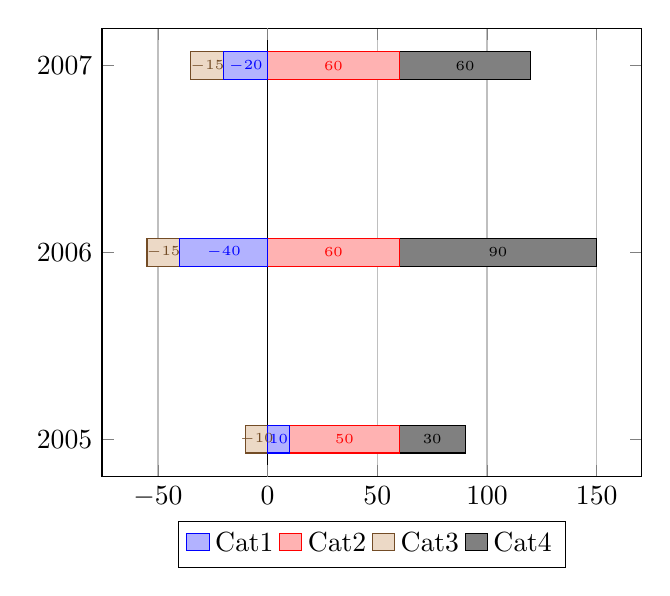
\begin{tikzpicture}
\pgfplotstableread{
Year    Cat1 Cat2      Cat3  Cat4
2005    10     50       -10    30
2006    -40     60       -15    90
2007    -20     60       -15    60
}\mytable
\begin{axis}[
  xbar stacked,
  % is default anyway:
  stack negative=separate,
  %
  /pgf/number format/1000 sep=,
  xmajorgrids,
  nodes near coords,
  nodes near coords style={font=\tiny},
  ytick distance=1,
  legend style={at={(0.5,-0.1)},anchor=north,legend
columns=-1},
  extra x ticks={0},
  extra x tick style={grid
style={black},xticklabel=\empty},
  ]
  \addplot table [x index=1,y=Year] {\mytable};
  \addplot table [x index=2,y=Year] {\mytable};
  \addplot table [x index=3,y=Year] {\mytable};
  \addplot table [x index=4,y=Year] {\mytable};
  \legend{Cat1,Cat2,Cat3,Cat4}
\end{axis}
\end{tikzpicture}


\end{document}

